\section{Basics}


\subsection{Poisson Reconstruction Overview}

Kazhdan, Bolitho and Hoppe described in \cite{Kazhdan06}
the Poisson Surface Reconstruction algorithm.
\cgal\ implements a variant of this algorithm which computes an implicit function
piecewise-linear in a 3D Delaunay triangulation instead of an octree.

This algorithm takes as input a 3D point set with oriented normals.
First, it builds a Delaunay triangulation and refines it (breaks bad tetrahedra, where {}``bad'' means
badly shaped or too big). The normal of Steiner points is set to zero.
Then it computes an indicator function f() piecewise-linear over the tetrahedra.
We solve the Poisson equation Laplacian(f) = divergent(normals field)
at each vertex of the triangulation via the TAUCS sparse linear solver.
Eventually, \cgal\ Surface Mesh Generator extracts the iso-surface {}``f() = median
of f() over the input points''.

% % Insert image poisson.jpg/eps
% \begin{center}
%     \label{Surface_reconstruction_3-fig-poisson}
%     % Image
%     \begin{ccTexOnly}
%         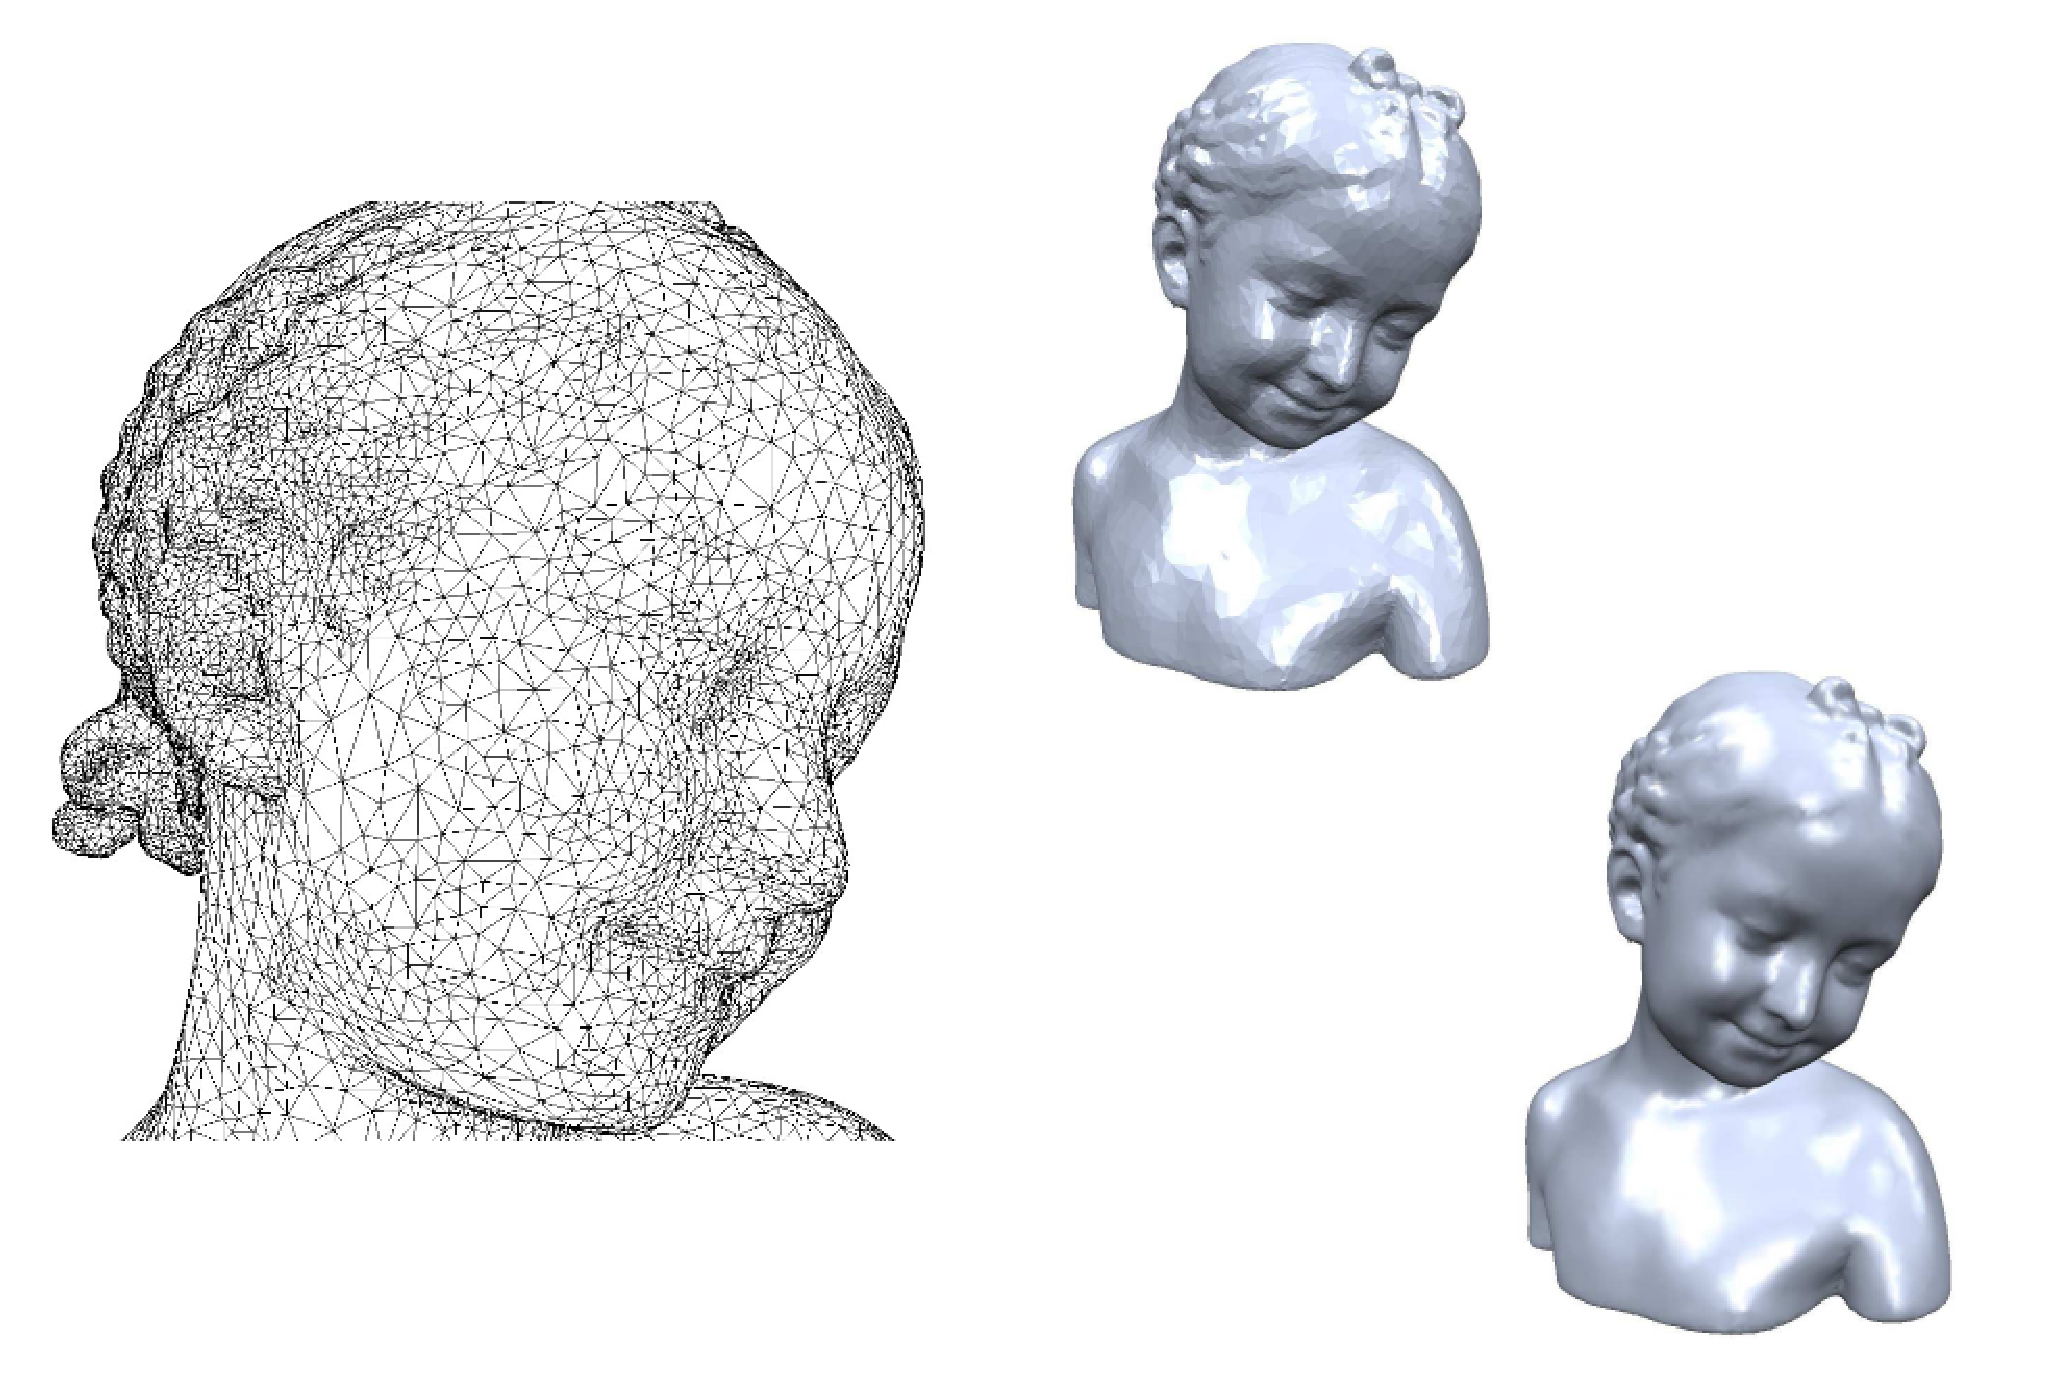
\includegraphics[width=0.9\textwidth]{Surface_reconstruction_3/poisson} % omit .eps suffix
%     \end{ccTexOnly}
%     \begin{ccHtmlOnly}
%         <img width="90%" border=0 src="./poisson.jpg"><P>
%     \end{ccHtmlOnly}
%     % Title
%     \begin{figure}[h]
%         \caption{Poisson reconstruction of the Bimba point set (from scanner)}
%     \end{figure}
% \end{center}


\subsection{Poisson Reconstruction API}

The class template declaration is:

template$<$  \\
class Gt,   \\
class \ccc{ReconstructionTriangulation_3}$>$   \\
class \ccc{Poisson_reconstruction_function};
\ccGlue
\begin{description}
\item[Parameters:]
\begin{description}
\item[Gt]Geometric traits class \item[\ccc{ReconstructionTriangulation_3}]3D Delaunay triangulation, model of \ccc{ReconstructionTriangulation_3} concept. \end{description}
\end{description}

The main constructor is:

\ccFunction{template<class InputIterator> Poisson_reconstruction_function(ReconstructionTriangulation_3& pdt, InputIterator first, InputIterator beyond);}
{
Create an implicit function from a point set. Insert the first...beyond point set into pdt and create a Poisson indicator function f() piecewise-linear over the tetrahedra of pdt.
Precondition: the value type of InputIterator must be convertible to \ccc{Point_with_normal}.
}
\ccGlue
\begin{description}
\item[Parameters:]
\begin{description}
\item[pdt]\ccc{ReconstructionTriangulation_3} base of the Poisson indicator function. \item[first]First point to add. \item[beyond]Past-the-end point to add. \end{description}
\end{description}

The main methods are:

\ccFunction{bool compute_implicit_function();}
{
You should call \ccc{compute_implicit_function}() once when points insertion is over. It computes the Poisson indicator function f() at each vertex of the triangulation by:\begin{itemize}
\item applying a Delaunay refinement to define the function inside and outside the surface.\item solving the Poisson equation Laplacian(f) = divergent(normals field) at each vertex of the triangulation via the TAUCS sparse linear solver. One vertex must be constrained.\item shifting and orienting f() such that f() = 0 on the input points, and f() $<$ 0 inside the surface.\end{itemize}
Return false on error.
}
\ccGlue
\ccFunction{FT f(const Point& p) const;}
{
Evaluate implicit function for any 3D point.
}
\ccGlue
\ccFunction{Point get_inner_point() const;}
{
Get point inside the surface.
}
\ccFunction{Sphere bounding_sphere() const;}
{
Get the surface's bounding sphere.
}

See details in  \\
\ccRefIdfierPage{CGAL::Poisson_reconstruction_function<GeomTraits, ReconstructionTriangulation_3>}


\subsection{Poisson Reconstruction Example}

\ccc{poisson_reconstruction_example.cpp} reads a point set, creates a Poisson implicit function
and reconstructs a surface.

\ccIncludeExampleCode{Surface_reconstruction_3/poisson_reconstruction_example.cpp}


